\chapter{System Design and Implementation}
\label{ch:method}

\section{Architecture and project boundary}

The implementation is divided into editor, resource, runtime and validation layers (\cref{fig:architecture}). The active demonstration project is separated from a synchronised distributable plugin template. Game scenes depend only on serialised resources and the runtime component; editor controls and live-debug presentation are not included in the game \ac{GUI}. This boundary prevents an authoring tool from becoming a hidden dependency of exported agent behaviour.

\begin{figure}[htbp]
    \centering
    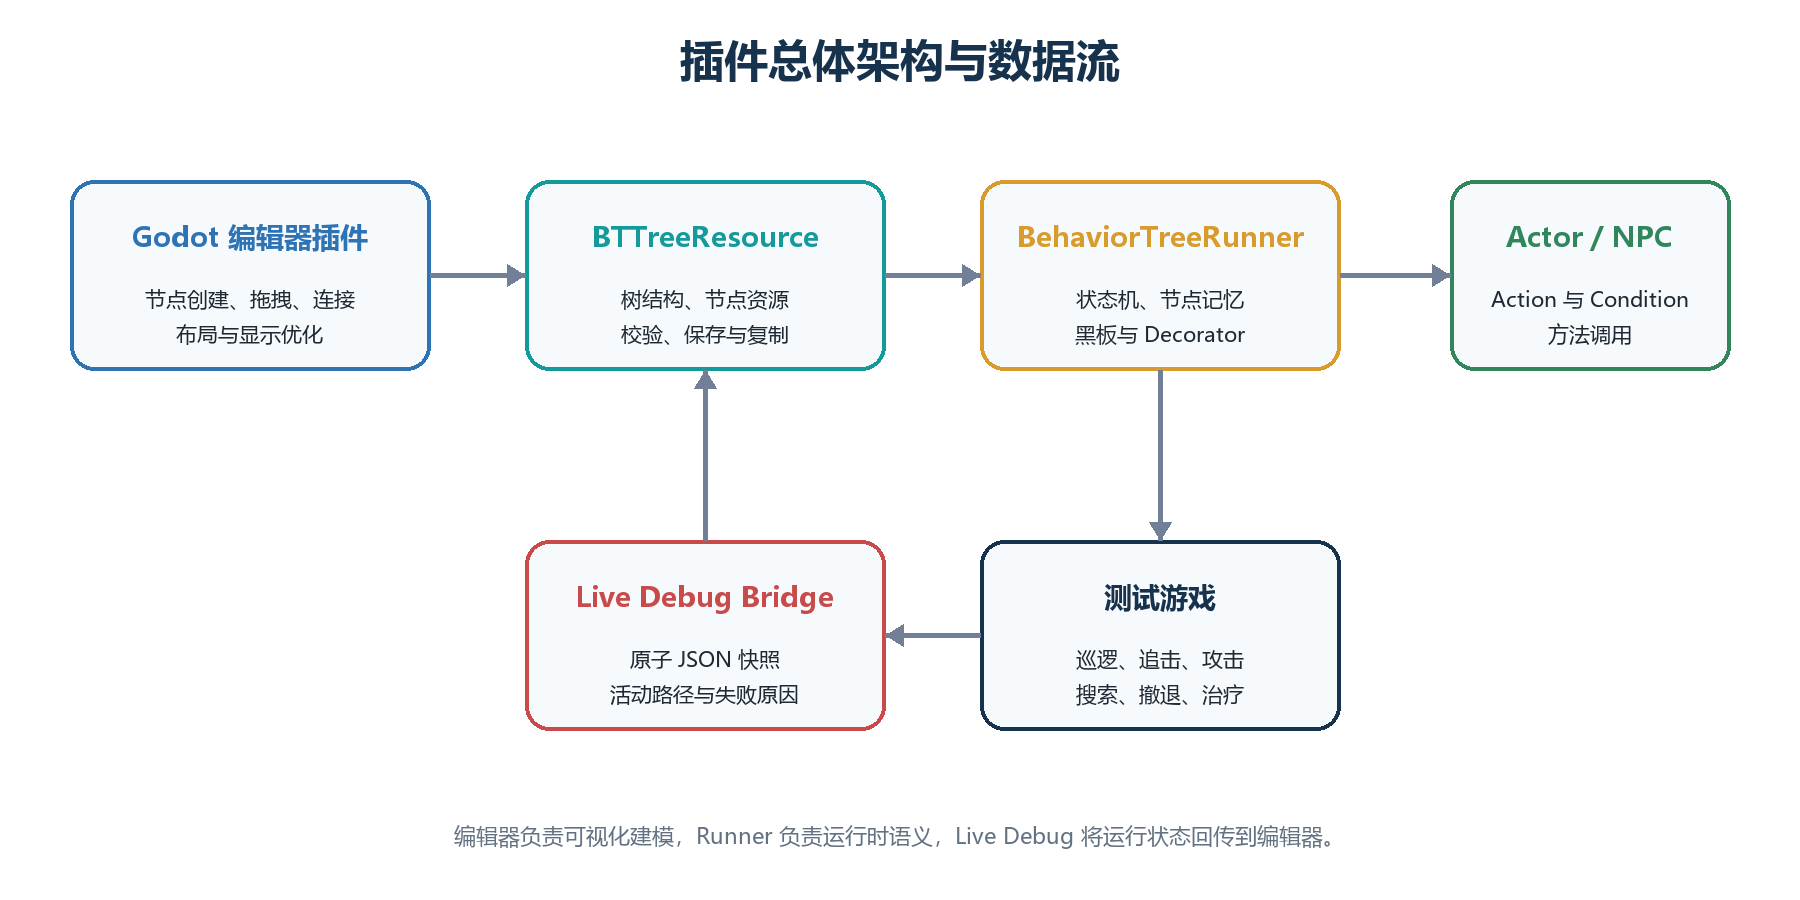
\includegraphics[width=\textwidth]{figures/architecture.png}
    \caption{Implemented plugin architecture and data flow between the Godot editor, behaviour-tree resource, runtime runner and actor.}
    \label{fig:architecture}
\end{figure}

\texttt{BTTreeResource} owns a root identifier, an array of node resources and an optional blackboard schema. \texttt{BTNodeResource} stores the type, title, description, parameters, graph position, ordinary parent and decorator owner. \texttt{BehaviorTreeRunner} executes a tree against an actor and dictionary blackboard. \texttt{BehaviorTreeComponent} exposes tree, actor path, tick mode and lifecycle as a reusable scene component. In the editor, \texttt{BTEditorView} coordinates the toolbar, graph, inspector, schema editor, history and live-debug panels; \texttt{BTGraphEdit} handles canvas interaction and custom connections; and \texttt{BTGraphNode} renders the card and status.

\section{Resource model and validation}

Ordinary hierarchy is represented by \texttt{parent\_id}. Decorators instead use \texttt{decorator\_parent\_id}, preventing them from becoming independent control-flow children. Child queries sort by graph X position, breaking ties by Y position. This makes the visible left-to-right sequence match execution order. Reordering a card therefore changes priority intentionally, while serialisation preserves the designer's layout.

Tree validation rejects missing roots, duplicate identifiers, invalid parent links, illegal decorator ownership and node-specific structural violations. A root must not have a parent; leaves cannot own ordinary children; a decorator must own a valid ordinary node; and required parameters must be present. Saving invokes the same validation used by tests, reducing the chance that an apparently valid graph fails only at runtime.

The blackboard schema contains typed entries for Boolean, integer, floating-point, string and \texttt{Vector2} values, together with defaults and a dynamic-key policy. Strict mode reports empty references and keys not declared by the schema. The Inspector presents declared keys in a typed picker while retaining free input for migration and dynamic use. A reverse index identifies which nodes reference a key and which declarations remain unused. Schema editing is integrated into tree-level undo/redo by deep-copying both nodes and schema entries.

\section{Runtime semantics}

Every tick returns \textsc{success}, \textsc{failure} or \textsc{running}. Node memory is indexed by node identifier and cleared on restart, tree replacement or branch interruption. The implemented semantics are summarised in \cref{tab:nodes}.

\begin{table}[htbp]
\centering
\caption{Implemented runtime node semantics.}
\label{tab:nodes}
\begin{tabular}{p{0.22\textwidth}p{0.68\textwidth}}
\toprule
Node & Behaviour \\
\midrule
Root & Executes its single ordinary child. \\
Sequence & Executes ordered children until one fails or runs; remembers a running index. \\
Selector & Executes ordered children until one succeeds or runs; remembers a running index. \\
Reactive Selector & Restarts priority checks each tick and interrupts a lower-priority running branch. \\
Random Selector & Chooses a child using a seedable generator and retains the choice while running. \\
Parallel & Ticks children and applies configurable success and failure thresholds. \\
Repeat & Repeats a child a fixed number of times or indefinitely, preserving count across ticks. \\
Wait & Accumulates delta time and succeeds after the configured duration. \\
Condition & Calls an actor predicate or compares a blackboard value. \\
Action & Calls an actor method and converts Boolean or status results into tree status. \\
\bottomrule
\end{tabular}
\end{table}

Action and actor-mode condition methods use a common signature: \texttt{method(blackboard, delta, node)}. The actor may return a tree status or a Boolean where appropriate. Missing methods fail safely and produce a debug reason rather than raising a fatal script error. Blackboard conditions support existence, non-existence, truth, falsity, equality, inequality and ordered numeric comparisons.

Decorators execute before or around their owner. Implemented modes include blackboard comparison, cooldown, time limit, invert, force result and repeat behaviour. Cooldown memory prevents immediate re-entry; time limit fails a running child after a threshold; invert exchanges success and failure; and force-result wrappers preserve running but replace the terminal result. Resetting a subtree clears decorator and child memory together.

\section{Editor authoring workflow}

The plugin registers a bottom editor panel. To avoid a permanent bank of node-creation buttons, a right-click canvas menu creates each node type at the requested graph position. Nodes can be moved, connected from a bottom square port to a top square port, disconnected through edge interaction, duplicated and removed. Composite nodes accept multiple children. Context menus expose common operations and subtree display commands. The tree selector shows the selected resource name rather than requiring users to manage a raw path field. All data-changing commands push a tree snapshot so undo and redo cover creation, deletion, movement, connection, parameter edits, schema edits and collapse state.

The inspector uses node-specific typed controls rather than requiring hand-written JSON for common fields. Actions choose a method name; conditions choose actor or blackboard mode, key, operator and comparison value; random, parallel, repeat and wait nodes expose their policies; decorators expose mode-specific parameters. An advanced JSON entry remains available for forward compatibility. Invalid JSON is parsed without emitting repeated red console errors, and the previous valid parameter object is retained until the input is repaired.

Connections required special handling because Godot's native \texttt{GraphEdit} curve uses side-oriented slots, whereas the intended behaviour-tree presentation uses vertical parent and child ports. In single-connection mode, the native persistent connection layer is hidden and a custom top-to-bottom edge is drawn. The native layer is temporarily restored during drag preview. Custom segment hit-testing preserves right-click disconnection and undo/redo. Disabling the feature restores native rendering, establishing a safe fallback.

Large-tree dragging avoids per-pointer resource notifications. During manual drag the card moves visually and only requests an edge redraw; the final resource position is synchronised on release. The undo snapshot is created after movement rather than on the latency-sensitive pointer-down path. Custom edge routes are cached by connection endpoints, off-screen edges are culled, unrelated pointer motion does not redraw the graph, and fisheye updates pause while dragging. These changes preserve the final position and one-step undo semantics while reducing repeated work.

\section{Live debugging and blackboard inspection}

The runner writes a compact snapshot containing actor identity, tree resource path, active node, ordered path, node statuses, failure reasons, blackboard values and schema information. A process-specific temporary file is atomically published to \path{res://.godot/behavior_tree_runtime_debug.json}. This avoids the editor reading a half-written JSON object. If a snapshot is truncated, the editor retains the previous complete state and recovers on the next publication.

The editor filters snapshots by the open tree resource and displays an active path, current leaf, path-summary row, failure menu and live blackboard table. Graph cards use status borders and annotations; non-active branches can be dimmed to alpha 0.24 while the active path remains at 1.0. The long runtime path and the current selection are separate scrollable rows, preventing overlap at the 1600 by 900 validation resolution. No corresponding overlay is present in the running game.

\begin{figure}[htbp]
    \centering
    
\includegraphics[width=0.92\textwidth]{figures/07_runtime_failure.png}
    \caption{Editor-only live debugging with the active path and a failure explanation attached to the relevant branch.}
    \label{fig:livedebug}
\end{figure}

\section{Large-tree display mechanisms}

Nineteen feature definitions are registered in a common switch system. State is persisted in a Godot \texttt{ConfigFile}; applying or disabling a feature calls a common refresh path. Switch combinations are tested by enabling features, rebuilding, disabling all features and checking for residue. The mechanisms are grouped below by purpose.

\subsection{Information-density control}

Compact cards reduce card width and height while retaining type encoding and a short title. Semantic zoom retains the same graph geometry but changes visible fields according to zoom level: low detail shows identity; higher detail reveals parameters, descriptions and decorator conditions. Type shape/icon encoding supplements colour, and an optional colourblind-safe palette provides redundant accessible cues.

\begin{figure}[htbp]
    \centering
    \begin{minipage}{0.48\textwidth}\centering
        
\includegraphics[width=\linewidth]{figures/01_baseline.png}\\[-1mm]
        \small (a) Baseline
    \end{minipage}\hfill
    \begin{minipage}{0.48\textwidth}\centering
        
\includegraphics[width=\linewidth]{figures/02_compact.png}\\[-1mm]
        \small (b) Compact cards
    \end{minipage}
    \caption{Full-detail baseline and compact-card presentation of the same behaviour tree.}
    \label{fig:compact}
\end{figure}

\subsection{Focus and structural reduction}

Fisheye magnifies the card under the pointer and nearby cards up to 1.20 times while retaining distant context. It changes internal size and font tokens rather than applying \texttt{GraphNode.scale}; centre compensation prevents the focus drifting to the right, and disable explicitly restores all presentation values. Subtree collapse hides descendants but reports their count and summaries from the next two levels. Subtree focus isolates a selected branch. Stable incremental layout attempts to reuse valid positions when rebuilding so unrelated branches do not jump.

\subsection{Navigation and overview}

Search matches title, type, description, method and decorator parameters; non-matches are dimmed and \texttt{F3}/\texttt{Shift+F3} navigate results. Breadcrumbs expose selected-node ancestors. Fit-to-view computes a scale sufficient for the complete graph, including a 0.10 minimum for stress trees. An enhanced 230 by 150 pixel minimap represents all nodes and the current viewport. Multi-column layout balances wide sibling groups while adding order cues so execution priority remains visible.

\subsection{Edge and execution representations}

Orthogonal routing replaces curves with right-angle segments. Edge bundling allows connections with a common direction to share a trunk, reducing repeated parallel geometry. Active-path highlighting, inactive-branch dimming, decorator badges, path summaries and failure annotations add execution-specific information without modifying the resource. Each of these remains optional because highlighting and edge styles can interact differently with tree density and user preference.

\section{Physical display experiment infrastructure}

The screen-size harness separates EDID physical surface from native resolution. A PowerShell inventory maps each active Windows display device to its EDID width and height, current desktop device and validated Godot screen index. For a display of width \(W_{cm}\) and height \(H_{cm}\), the controlled canvas is
\[
W_c=35W_{cm}, \qquad H_c=35H_{cm},
\]
where \(W_c\) and \(H_c\) are logical canvas units. The graph cards retain the same logical dimensions, so a larger physical surface supplies proportionally more controlled canvas rather than inheriting a device's arbitrary pixel density.

The real-renderer harness moves the experiment window to the requested display, instantiates the editor in the normalised \texttt{SubViewport}, applies the same deterministic tree and display conditions, and records physical metadata with every row. Each session has an immutable device inventory and separate per-device raw CSV, summary, manifest, log and screenshots. A combined analysis regenerates the paired screen-size table and input SHA-256 manifest; a new monitor is recorded under a new session rather than replacing existing evidence.

\section{Runtime topology cache}

Uncached runtime queries repeatedly scan the node array to find an identifier, gather a parent's children and gather an owner's decorators. The optional cache builds three indexes: node ID to resource, parent ID to ordered children, and owner ID to ordered decorators. Dynamic condition and action results are never cached.

A naïve cache that checks only resource instance and node count is unsafe when a tree is edited in place without changing its size. The final implementation computes an exact topology signature once per external tick. It contains root ID, node count, every node resource instance, node ID, parent ID, decorator owner and X/Y ordering position. A changed signature rebuilds all indexes. Recursive execution reuses the already validated cache for the remainder of that tick. This preserves mutation safety at the cost of an \(O(n)\) validation scan, a deliberate correctness--performance trade-off.

\section{Demonstration game}

The complex 2D arena provides behavioural evidence beyond synthetic trees. The player can move, jump, climb ladders, perform melee attacks, dash, heal and briefly cloak. Three guards run behaviour-tree components against a shared 241-node resource. At low health a guard retreats and heals; reactive defence answers the player's live attack window; directional melee checks range and facing; ranged suppression aims and spawns a visible projectile; obstacle sensing selects a jump rather than walking into a crate; and an elevated detected player near a ladder selects climbing. Lower-priority branches cover pressure, coordinated chase, last-known-position search, return, layered patrol and idle variation. Detection uses hysteresis: a visible player is acquired within 330 pixels and released beyond 460 pixels, preventing rapid oscillation at a single threshold.

The game intentionally uses simple generated shapes and texture changes rather than animation-heavy art. This keeps the experimental emphasis on decision logic and makes automated state assertions reliable.
